\section{State Diagram}\label{section:state-diagram}

A state diagram shows the different states the program can be in and the options the user can perform to change the state of the program.
State diagrams are useful models for designing the interfaces. 
The state diagram for this project can be seen in \figref{figure:state-diagram}, which includes all the transitions and states for the program. 

\begin{figure}[h]
	\centering
	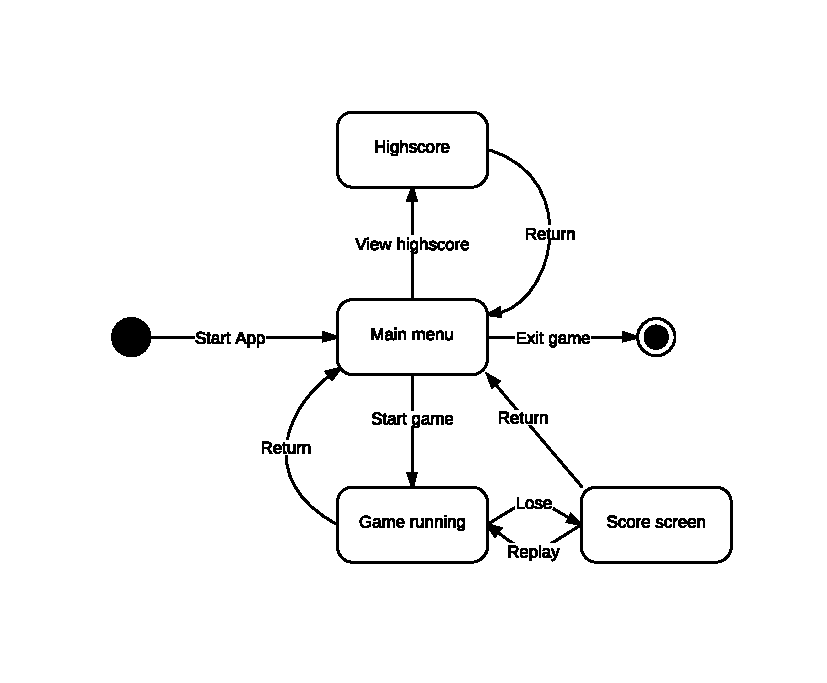
\includegraphics[trim = 0cm 1.5cm 0cm 1.5cm, clip, scale = 1]{media/design/state-diagram.pdf}
	\caption{Application state diagram.}
	\label{figure:state-diagram}
\end{figure}

Initially, the user will launch the application, which will present the \textit{Main menu}.
From here, the user can press the buttons \textit{Start game}, \textit{View highscore}, or \textit{Exit game}. 
Start game will render the game to begin, and the application will now be in the state \textit{Game running}, it will remain in this state until the user loses the game, or the user chooses to \textit{Return} to the Main menu.
When the user loses the game, a \textit{Score screen} will appear, allowing the user to \textit{Replay} or Return to the Main menu. 
Furthermore, when a user loses a game, the achieved score can be submitted to the highscore, which can be viewed in the \textit{Highscore} state.
The Highscore state can be accessed from the Main menu.